\scanpage{152}\mspage{7}%
A) Le formalisme des $Rf_!, f^!$ (combiné à $Rf_*, Lf^{\unsure{\alpha|*}}$, $\overset{\mathbb{L}}{\otimes}$ et $\mathbb{R}\mathrm{Hom}$, ``les six opérations'') porte implicitement en son sein la définition de l'homologie et l'identité essentielle entre \unsure{fonctions} homologiques et cohomologiques. \deleted{\unsure{E}} On dispose pour le moment de ce formalisme pour les faisceaux quasi-cohérents sur les schémas -- séminaire Hartshorne -- pour les espaces top. et les faisceaux de coeff. arbitraires dessus -- Verdier, exposé Bourbaki -- et en coh. étale des schémas pour les coefficients ``discrets'' \inserted{(de torsion ou ``$l$-adiques'')}
% Source guide below the parenthetic addition: long upper arm, left downward bend, and short left foot; no arrowhead. The downward leg passes beside premiers and through the interlinear-note zone.
\figure{\begin{tikzpicture}[x=0.01cm,y=-0.01cm,line cap=round,line join=round]
\draw[line width=0.55pt] (626,3) .. controls (630,9) and (629,12) .. (621,12) -- (47,16) .. controls (22,16) and (16,21) .. (16,46) -- (15,109) -- (4,112);
\end{tikzpicture}}
\uline{premiers a\unsure{\.{u}|u}x \deleted{\unsure{la|le}} car. résiduelles} -- SGA 5 --
% The right guide lies above the added analytic case and descends from after SGA 5 into the space above the names. Its semicolon is reproduced inside the bend, not assigned an invented baseline order.
\figure{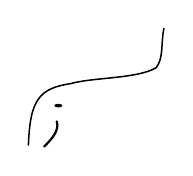
\begin{tikzpicture}[x=0.02cm,y=-0.02cm,line cap=round,line join=round]
\draw[line width=0.55pt] (89,2) .. controls (87,11) and (89,21) .. (84,27) .. controls (72,34) and (44,33) .. (30,37) .. controls (10,40) and (4,47) .. (3,76);
\fill (22,51) ellipse [x radius=2.6,y radius=1.15];
\draw[line width=0.8pt] (21,61) .. controls (23,67) and (17,73) .. (13,77);
\end{tikzpicture}}
\inserted{enfin pour les faisc. coh. sur les espaces analytiques -- Verdier-\unsure{Ruget|Rüget} --}
% The addition is slightly slanted in the source.
(Le formalisme reste à développer dans le contexte cristallin, et en car. $0$ dans le contexte des modules stratifiés \inserted{à singularités}
% Guide immediately below singularités: the left end bends down just before the baseline à la; the long arm continues rightward beneath the added word.
\figure{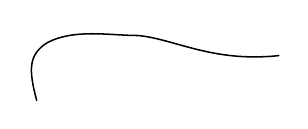
\begin{tikzpicture}[x=0.015cm,y=-0.015cm,line cap=round,line join=round]
\draw[line width=0.55pt] (8,61) .. controls (1,35) and (1,22) .. (17,12) .. controls (40,0) and (70,6) .. (94,6) .. controls (125,9) and (157,29) .. (213,23);
\end{tikzpicture}}
à la Deligne, avec éventuellement -- sur le corps $\mathbb{C}$ -- des structures de Hodge à la clef, enfin dans le contexte des motifs ; je suis persuadé qu'il est présent
% The small doubtful point stands below the beginning of un, rather than after the word.
\makebox[0pt][l]{\hspace{0.1em}\raisebox{-1.4ex}[0pt][0pt]{\unsure{.}}}un peu partout encore -- partout, peut-être, où il y a un formalisme de nature cohomologique.) Travaillant en coh. étale sur un schéma \inserted{séparé}
% Guide immediately below séparé: curved left descent before de, rising arm, and small terminal hook at upper right.
\figure{\begin{tikzpicture}[x=0.02cm,y=-0.02cm,line cap=round,line join=round]
\draw[line width=0.55pt] (14,70) .. controls (3,55) and (3,40) .. (19,34) .. controls (40,25) and (82,19) .. (105,9) .. controls (114,5) and (110,0) .. (102,3);
\end{tikzpicture}}
de t.f. sur un corps $k$, disons, avec un anneau de coeff. $\Lambda$ de torsion premier à \unsure{la} \unsure{car}
% The last baseline is cut by the lower edge; no final punctuation is recoverable.
% archive sheet number: 152
